\section{Critical Calibration Method}

\subsection{Theory}
The calibration of control rods in a reactor is crucial for understanding their reactivity worth. This can be accomplished using the in-hour and point kinetics equations to relate the time required to increase power by a factor to the reactivity.

\paragraph{Reactivity and Reactor Period}
The relationship between reactivity ($\rho$) and the reactor period ($T$) is fundamental in control rod calibration. The point kinetics equations describe this relationship:
\begin{equation}
    \frac{dP}{dt} = \frac{\rho - \beta}{\Lambda}P + \sum_{i=1}^6 \lambda_i C_i
\end{equation}
\begin{equation}
    \frac{dC_i}{dt} = \frac{\beta_i}{\Lambda}P - \lambda_i C_i
\end{equation}
where:
\begin{itemize}
    \item $P$ is the reactor power,
    \item $\rho$ is the reactivity,
    \item $\beta$ is the delayed neutron fraction,
    \item $\Lambda$ is the prompt neutron lifetime,
    \item $\beta_i$ and $\lambda_i$ are the delayed neutron fractions and decay constants for each of the six precursor groups,
    \item $C_i$ is the concentration of the $i$-th delayed neutron precursor group.
\end{itemize}

The in-hour equation provides a direct link between the reactor period and reactivity:
\begin{equation}
    \rho = \frac{\Lambda}{T} + \sum_{i=1}^6 \frac{\beta_i \lambda_i}{1 + \lambda_i T}
\end{equation}
This equation allows the calculation of reactivity based on measurements of $T$. For small reactivity, we approximate $\rho$ as:
\begin{equation}
    \rho \approx \frac{\Lambda}{T} + \sum_{i=1}^6 \frac{\beta_i \lambda_i}{1 + \lambda_i T}
\end{equation}

\subsection{Experiment}
We calibrated the REG control rod of the TRIGA reactor. Calibration is necessary because the reactivity introduced by a control rod is not directly proportional to its insertion depth; instead, effectiveness varies with insertion depth, as illustrated in the following graphs:

\begin{figure}[h]
    \centering
    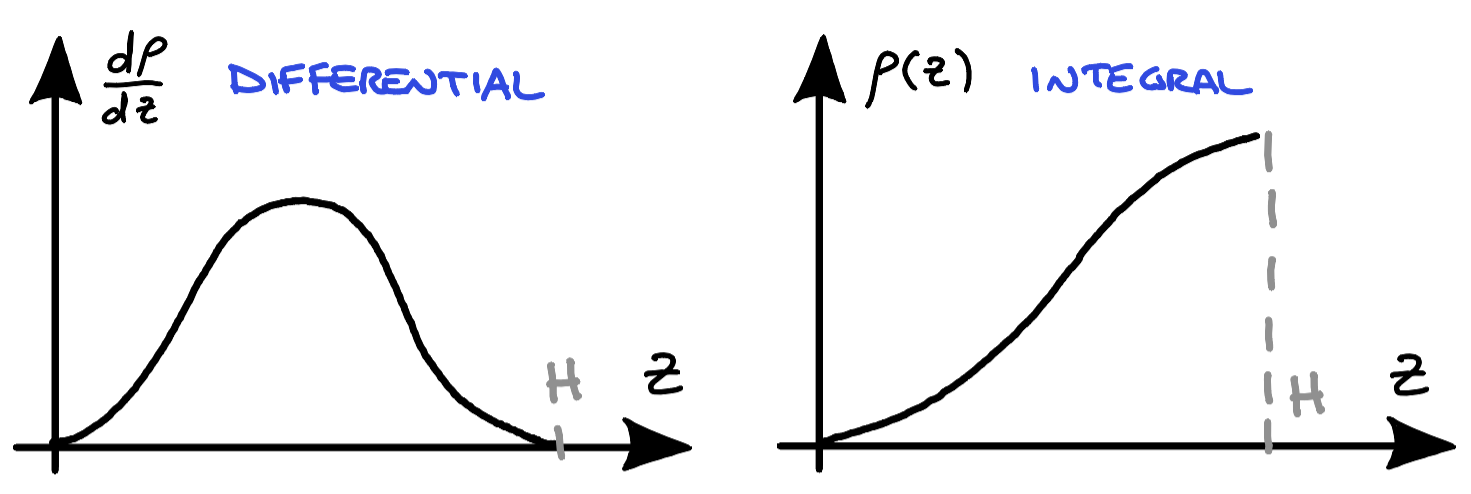
\includegraphics[width=0.75\linewidth]{CR_2.png}
    \caption{Differential and Integral reactivity curves}
\end{figure}

\textbf{Cold and clean conditions:} The experiment was conducted under these conditions to avoid external effects such as poisons and thermal feedback.

\begin{tcolorbox}[boxstyle2, title=PRO vs CONS]
    \textbf{Advantages}:
    \begin{itemize}
        \item Absolute method: results are independent of other factors, including the position of other control rods
        \item High accuracy of results 
    \end{itemize}
    \textbf{Disadvantages}: 
    \begin{itemize}
        \item Time-intensive, as calibration is required for each control rod
        \item Reactor remains in supercritical condition during measurements, raising safety concerns for non-TRIGA reactors
    \end{itemize}
\end{tcolorbox}

\subsection{Formulas}
The total reactivity worth ($\Delta \rho _{TOT}$) is given by:
\begin{equation}
    \Delta \rho _{TOT} = \Delta \rho _{SM} + \Delta \rho _{EX}
\end{equation}
where $\Delta \rho _{SM}$ is the shutdown margin and $\Delta \rho _{EX}$ is the reactivity excess.

Shutdown Margin:
\begin{equation}
    \Delta \rho _{SM} = \rho_i (\text{Criticality}) - \rho_i (\text{Fully IN}) 
\end{equation}
Reactivity excess:
\begin{equation}
    \Delta \rho _{EX} = \rho_i (\text{Fully OUT}) - \rho_i (\text{Criticality})
\end{equation}

\subsection{Procedure}
\begin{enumerate}
    \item Incrementally raise the REG rod and measure the time required for power increases.
    \item Adjust the shim rod to maintain criticality.
    \item Repeat until the REG rod is fully withdrawn.
\end{enumerate}

\subsection{Conclusion}
The critical calibration method provides precise reactivity measurements but requires careful handling as the reactor remains in a supercritical state. This method allows for detailed control rod worth assessment and is valuable for reactor safety and efficiency.